\chapter{METODOLOGÍA Y MARCO TECNOLÓGICO}

El presente capítulo describe el enfoque metodológico y las decisiones tecnológicas adoptadas para el desarrollo del sistema Bebras Bolivia. En primer lugar, se analizan plataformas nacionales de referencia con el propósito de identificar patrones de arquitectura, módulos funcionales y criterios de diseño reutilizables. Posteriormente, se examina la naturaleza de los sistemas de gestión de concursos en línea, distinguiéndolos de otras plataformas educativas y precisando los requisitos operativos que condicionan su implementación.

Finalmente, se presentan las herramientas y tecnologías seleccionadas para la construcción del sistema, justificando su elección en función de criterios de rendimiento, mantenibilidad, coherencia de pila y adecuación al contexto del proyecto. Esta exposición metodológica y tecnológica permite fundamentar la solución propuesta no solo desde el punto de vista conceptual, sino también desde su viabilidad práctica e implementación efectiva.

\section{ANÁLISIS COMPARATIVO DE PLATAFORMAS BEBRAS DE REFERENCIA}

Con el propósito de fundamentar las decisiones de diseño funcional, arquitectónico y de interfaz del sistema propuesto para Bebras Bolivia, se realizó un análisis comparativo sobre un conjunto de implementaciones nacionales del Desafío Bebras. Este análisis no se limitó a una descripción general de los sitios o repositorios disponibles, sino que buscó identificar de manera sistemática, a partir de la observación de su funcionamiento y de la información técnica pública disponible, los componentes, patrones de organización, módulos funcionales y estrategias de interacción más relevantes de cada plataforma revisada.

La selección de los casos de estudio respondió a criterios complementarios: disponibilidad de código fuente o información técnica pública, grado de madurez de la implementación, representatividad dentro del ecosistema Bebras y utilidad como referencia para el contexto boliviano. A partir de esta revisión, fue posible reconocer fortalezas particulares en cada plataforma y extraer de ellas los elementos más valiosos para la definición de la propuesta tecnológica del presente trabajo. En consecuencia, el análisis realizado no tuvo como finalidad replicar una solución existente, sino sintetizar buenas prácticas dispersas en distintas implementaciones nacionales para integrarlas en un sistema propio, coherente con los requerimientos de Bebras Bolivia.

\subsection{Plataforma de Francia --- Castor Informatique}

La implementación francesa, \emph{Castor Informatique}, mantenida por France-IOI, constituye una de las referencias más consolidadas dentro del ecosistema Bebras y dispone de código fuente accesible públicamente \parencite{bebrasfrancia}. El análisis de su estructura permitió identificar una separación clara entre módulos de concurso, maestros y preguntas, así como una estrategia orientada a optimizar la entrega de contenido mediante generación o compilación previa de materiales de prueba.

Desde la perspectiva de este análisis, el principal aporte de esta plataforma radica en su eficiencia para servir contenido y en la organización clara de sus componentes funcionales. Para Bebras Bolivia, esta referencia resultó especialmente útil en la definición de estrategias de entrega de contenido y en la inspiración de un esquema modular para separar áreas públicas, administrativas y de evaluación.

\subsection{Plataforma de Bélgica --- Rasbeb2}

La plataforma belga \emph{Rasbeb2}, disponible bajo licencia MIT \parencite{bebrasbelgica}, presenta una arquitectura orientada a la gestión integral del concurso. Su implementación en Java y su organización por módulos administrativos, tareas interactivas y documentación permitieron identificar una estructura robusta para el manejo de procesos internos del sistema.

El principal valor extraído de esta plataforma fue su diseño modular aplicado al flujo del concurso, particularmente en la separación entre inscripción, administración, ejecución y evaluación. Aunque no se adoptó su base tecnológica, su organización interna aportó criterios relevantes para estructurar el sistema Bebras Bolivia desde una lógica funcional más que desde una lógica de simple desarrollo web.

\subsection{Plataforma de Perú --- Bebras Perú}

La plataforma de Bebras Perú \parencite{bebrasperu} ofrece una referencia importante desde el punto de vista comunicacional e institucional. Su sitio prioriza la presentación pública de información para maestros, instituciones educativas y participantes, organizando con claridad niveles, recursos, orientaciones y mecanismos de inscripción.

A partir del análisis de esta plataforma, se identificó como fortaleza principal la claridad en la arquitectura de información orientada a usuarios no técnicos. Este aspecto fue considerado especialmente valioso para el diseño del sitio informativo de Bebras Bolivia, ya que evidencia la necesidad de estructurar el contenido de manera diferenciada para instituciones educativas, maestros, estudiantes y familias.

\subsection{Plataforma de Estados Unidos --- Bebras Computing Challenge}

La plataforma de \textcite{bebraseeuu} combina un entorno de práctica abierta con acceso a tareas de ediciones anteriores y un espacio de gestión dirigido a responsables institucionales. Su interfaz organiza de forma clara las categorías, el formato del concurso y los mecanismos de participación, al mismo tiempo que ofrece una experiencia de resolución de ejercicios bien definida.

Desde el análisis realizado, su principal aporte fue el modelo de interacción del módulo de ejercicios, especialmente en aspectos como la presentación del problema, la navegación entre tareas, la retroalimentación al usuario y la integración entre práctica y evaluación. Estos elementos sirvieron como referencia directa para definir la experiencia de uso esperada en el módulo de resolución de tareas de Bebras Bolivia.

\subsection{Síntesis de aportes extraídos del análisis comparativo}

El análisis comparativo de las plataformas revisadas permitió concluir que no existe una única implementación que resuelva de manera integral todos los requerimientos identificados para Bebras Bolivia. Sin embargo, cada una de las referencias estudiadas aporta fortalezas concretas que pueden ser integradas en una propuesta propia. En este sentido, el presente proyecto no se plantea como una réplica de ninguna plataforma existente, sino como una síntesis de buenas prácticas funcionales, arquitectónicas y de interfaz observadas en distintas implementaciones nacionales del ecosistema Bebras.

\begin{table}[H]
\centering
\caption[Elementos recuperados de plataformas Bebras de referencia]{Elementos recuperados mediante el análisis comparativo de plataformas Bebras de referencia y su aplicación en Bebras Bolivia}
\label{tab:retro_bebras}
\renewcommand{\arraystretch}{1.25}
\begin{tabular}{|p{3.5cm}|p{4.8cm}|p{6cm}|}
\hline
\textbf{Plataforma} & \textbf{Elemento rescatado} & \textbf{Aplicación} \\ \hline
Castor Informatique & Separación entre concurso, maestros y banco de preguntas; publicación eficiente de contenidos & Base para dividir el sistema en módulos administrativos, académicos y de evaluación, y para orientar la entrega optimizada de tareas y recursos \\ \hline
Rasbeb2 & Organización modular del flujo del concurso y soporte para tareas interactivas & Referencia para estructurar los procesos de inscripción, ejecución, corrección y administración del concurso dentro del CMS \\ \hline
Bebras Perú & Arquitectura de información clara para maestros, instituciones y postulantes & Base para diseñar el sitio informativo y ordenar la comunicación institucional según tipo de usuario \\ \hline
Bebras Computing Challenge & Presentación de tareas, práctica previa y navegación entre ejercicios & Referencia para definir la experiencia del participante en el módulo de resolución de tareas y práctica \\ \hline
\end{tabular}
\end{table}

\section{SISTEMAS DE GESTIÓN DE CONCURSOS EN LÍNEA}

Un sistema de gestión de concursos en línea es una plataforma web que administra de manera integral el ciclo de vida de una competencia: el registro de participantes e instituciones, la configuración y distribución de pruebas, la ejecución controlada de exámenes en sesiones con tiempo limitado, la evaluación automática de respuestas y la publicación de resultados. Este tipo de sistemas se articula en torno a tres funciones esenciales: la autenticación segura de los participantes, la gestión del banco de preguntas y el motor de evaluación automática. Estos tres componentes están presentes en todas las implementaciones nacionales de Bebras analizadas y definen igualmente los módulos centrales del sistema desarrollado en este proyecto.

A diferencia de un sistema de gestión de aprendizaje (\textit{Learning Management System}, LMS) de propósito general, un sistema de gestión de concursos educativos debe garantizar condiciones equivalentes para todos los participantes durante la ejecución de la prueba: disponibilidad simultánea para múltiples sesiones concurrentes, control estricto del tiempo por participante y registro confiable de respuestas ante posibles interrupciones de conectividad. Estos requisitos condicionan directamente las decisiones de arquitectura del sistema propuesto.

La distinción funcional entre un sistema de gestión de concursos y un LMS se ilustra en la Figura~\ref{fig:cms_vs_lms}.

\begin{figure}[htbp]
    \centering
    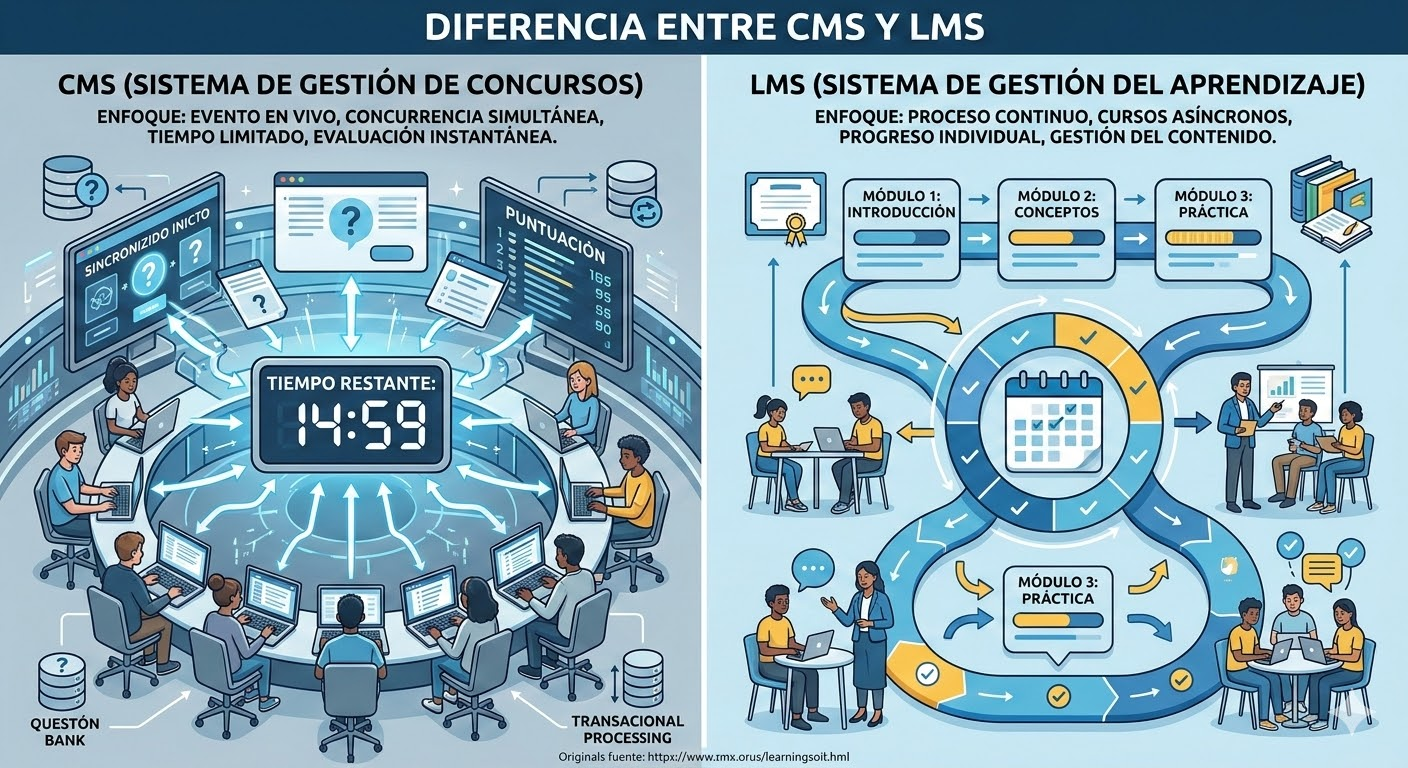
\includegraphics[width=0.70\textwidth]{assets/cms_vs_lms.jpg}
    \caption[Comparación entre CMS y LMS]{Comparación conceptual entre un \textit{Contest Management System} y un \textit{Learning Management System}}
    \label{fig:cms_vs_lms}
\end{figure}

\section{METODOLOGÍA DE ANÁLISIS Y DISEÑO}

La metodología adoptada en este trabajo combina revisión documental, análisis comparativo de plataformas de referencia y definición de una arquitectura ajustada a los requisitos funcionales y no funcionales del proyecto. En una primera etapa, se realizó una revisión de literatura especializada sobre pensamiento computacional, el modelo Bebras y la construcción de tareas educativas de informática. En una segunda etapa, se analizaron distintas plataformas nacionales de Bebras con el fin de identificar módulos recurrentes, patrones de interacción y decisiones arquitectónicas relevantes.

Sobre la base de este análisis, se procedió a definir los módulos que conforman la propuesta tecnológica para Bebras Bolivia: gestión de contenido y sitio informativo, gestión de competencias, registro de participantes y evaluación digital e imprimible. Finalmente, se seleccionó una pila tecnológica coherente con los requerimientos de rendimiento, mantenibilidad y escalabilidad identificados durante el proceso.

\subsection{Extreme Programming (XP)}

El desarrollo del presente proyecto adoptó \textit{Extreme Programming} (XP) como metodología ágil de referencia. XP fue propuesto por \textcite{beck2004} como un enfoque orientado a equipos pequeños que trabajan sobre requisitos cambiantes, priorizando la entrega continua de software funcional y la incorporación sistemática de retroalimentación. Estas características lo hacen especialmente adecuado para un proyecto de grado en el que el desarrollo avanza de forma incremental, con revisiones periódicas por parte del supervisor y ajustes continuos al alcance y al diseño del sistema.

La elección de XP como metodología de referencia se fundamenta en una comparación con otras alternativas ampliamente utilizadas. Scrum, aunque popular en equipos de desarrollo profesional, presupone roles diferenciados \textit{Product Owner}, \textit{Scrum Master} y equipo de desarrollo y una estructura de ceremonias formales que no se corresponden con el equipo reducido de dos desarrolladores que conforma este proyecto \parencite{schwaber2020}. Kanban, por su parte, ofrece flexibilidad en la gestión del flujo de trabajo, pero carece de los mecanismos de planificación por valores y retroalimentación continua que XP incorpora de manera explícita \parencite{anderson2010}. En contraste, XP está diseñado para contextos donde el equipo es reducido, los requisitos evolucionan durante el desarrollo y la calidad del software es una prioridad sostenida a lo largo de todo el proceso.

XP se articula en torno a cinco valores fundamentales que orientan las decisiones de diseño y desarrollo \parencite{beck2004}. La \textit{comunicación} se manifiesta en este proyecto a través del diálogo continuo con el supervisor, que permite alinear expectativas y corregir el rumbo en cada ciclo de avance. La \textit{simplicidad} guía las decisiones de arquitectura y diseño de módulos, priorizando soluciones directas y mantenibles sobre implementaciones sobredimensionadas. La \textit{retroalimentación} opera como mecanismo central de validación: cada entrega parcial es revisada y genera insumos concretos para la iteración siguiente. La \textit{valentía} se refleja en la disposición a refactorizar o rediseñar componentes cuando el análisis lo justifica, sin preservar decisiones técnicas por inercia. Finalmente, el \textit{respeto} se traduce en el cuidado por producir un sistema coherente, bien documentado y sostenible más allá del alcance inmediato del proyecto.

De las prácticas que XP propone, este proyecto incorpora de manera explícita el desarrollo iterativo e incremental, la integración continua de retroalimentación como insumo de corrección, la validación sostenida de decisiones de diseño y arquitectura y la programación en pareja, práctica que resulta especialmente adecuada para un equipo de dos desarrolladores. No se adoptaron, en cambio, prácticas pensadas para equipos numerosos, como la propiedad colectiva del código a gran escala, dado que el proyecto es desarrollado por un equipo de dos personas con responsabilidades claramente delimitadas. Esta selección de prácticas de XP es consistente con lo señalado por \textcite{shore2021}, quienes reconocen que los equipos pueden adoptar un subconjunto coherente de prácticas XP sin comprometer los principios fundamentales de la metodología.

Siguiendo el principio de iteraciones cortas de duración fija propio de XP, el desarrollo se organizó mediante \textit{timeboxing}. En XP, las iteraciones suelen mantenerse dentro de rangos breves, comúnmente entre una y tres semanas, con el propósito de entregar incrementos verificables y recibir retroalimentación frecuente. Para el presente proyecto se adoptaron iteraciones de tres semanas, debido a que el desarrollo se realizó en paralelo con actividades de análisis, documentación, validación con el supervisor y refinamiento funcional del producto.

Dado que los módulos del sistema presentan distinta extensión y complejidad, no existe una correspondencia directa entre un módulo y una única iteración. En lugar de extender la duración de una iteración para acomodar un módulo de mayor tamaño, cada módulo se desarrolla a lo largo del número de iteraciones que requiera, manteniendo invariable la caja de tiempo de tres semanas.

\subsection{Diseño centrado en el usuario e interacción persona computadora}

Complementariamente a XP, el desarrollo del sistema incorporó principios de diseño centrado en el usuario (\textit{User-Centered Design}, UCD), definidos en la norma \textcite{iso9241210}. Este enfoque establece que las decisiones de diseño deben fundamentarse en el conocimiento de los usuarios, sus tareas y su contexto de uso, con el propósito de producir sistemas que sean utilizables, accesibles y adecuados a las necesidades reales de quienes los emplean.

La pertinencia de este enfoque en el presente proyecto se deriva de la diversidad de perfiles de usuario que interactúan con el sistema. La arquitectura funcional contempla tres actores principales: el \textbf{administrador u organizador}, responsable de la configuración global del concurso y de la administración del contenido; el \textbf{maestro}, encargado de articular la participación de su unidad educativa o grupo de estudiantes; y el \textbf{estudiante}, cuya interacción se concentra en el acceso y resolución de la prueba. Cada actor presenta competencias digitales, objetivos y contextos de uso diferentes, por lo que las decisiones de interfaz no pueden abordarse de manera uniforme. Las definiciones de navegación, estructura de información y presentación de contenido se orientaron en función de los requisitos específicos de cada rol, tomando como referencia los principios de usabilidad descritos por \textcite{norman2013}.

El módulo de resolución de tareas merece una atención particular desde la perspectiva de la interacción persona computadora (\textit{Human-Computer Interaction}, HCI). Al tratarse del componente con el que interactúan directamente los estudiantes, el grupo de usuarios con menor experiencia digital y mayor heterogeneidad etaria dentro del sistema, su diseño debe atender criterios de usabilidad, claridad visual y accesibilidad de manera rigurosa. \textcite{preece2015} señalan que el diseño de interfaces para usuarios con perfiles cognitivos y etarios diversos exige una atención especial a la carga cognitiva, la consistencia visual y la retroalimentación inmediata ante las acciones del usuario. En este contexto, aspectos como el contraste visual, la legibilidad tipográfica, la navegación entre tareas y la presentación del tiempo disponible no son decisiones estéticas, sino funcionales: condicionan directamente la capacidad del estudiante para concentrarse en la resolución del problema sin ser obstaculizado por la interfaz misma.

Adicionalmente, el sistema debe considerar criterios de accesibilidad web definidos por las \textit{Web Content Accessibility Guidelines} (WCAG) \parencite{w3c2023}, que establecen estándares internacionales para garantizar que el contenido digital sea perceptible, operable, comprensible y robusto para usuarios con distintas capacidades. Dado que el concurso está dirigido a estudiantes de nivel primario y secundario en un contexto educativo diverso, la accesibilidad no es un complemento opcional sino un requisito de equidad: un sistema que no puede ser utilizado eficazmente por todos los participantes compromete la validez misma del concurso.

\section{MARCO TECNOLÓGICO}

El objetivo técnico central de este proyecto es el desarrollo de un sistema capaz de administrar de extremo a extremo el ciclo de vida del Desafío Bebras Bolivia: inscripción de instituciones y participantes, configuración y distribución de exámenes, ejecución controlada de pruebas en línea, registro automático de respuestas y consulta de resultados. A este sistema se suma un sitio informativo con capacidades propias de gestión de contenido, orientado a la comunicación institucional del desafío. La selección de tecnologías responde a criterios de rendimiento, coherencia de pila y mantenibilidad a largo plazo, considerando que ambos módulos deben operar de manera integrada sobre el mismo entorno de ejecución.

\subsection{Astro}

Astro fue seleccionado para el sitio informativo por su enfoque en rendimiento y generación de contenido estático. \textcite{astro} destaca su modelo \textit{server-first} y la \emph{Islands Architecture}, que hidrata solo los componentes interactivos y reduce JavaScript en cliente. Además, su integración con \textit{Content Collections} permite administrar contenido institucional de forma tipada y mantenible, en coherencia con la pila basada en Bun.

\subsection{Bun}

Bun se utiliza como entorno de ejecución unificado para JavaScript y TypeScript en el proyecto. \textcite{bun} lo describe como una alternativa de alto rendimiento que integra \textit{runtime}, gestor de paquetes y herramientas de desarrollo en una sola tecnología. Esta unificación simplifica la operación del sistema y reduce tiempos de ejecución y despliegue frente a cadenas de herramientas separadas.

\subsection{Express}

Express se eligió para la capa API del sistema por su arquitectura modular basada en \textit{middleware}. \textcite{express} resalta su flexibilidad para estructurar rutas, validaciones y control de errores sin imponer una arquitectura rígida. Esto ofrece una base adecuada para implementar flujos como autenticación, gestión de sesiones de examen y registro de respuestas dentro de un sistema de este tipo.

\subsection{Prisma ORM}

Prisma ORM se adoptó para el acceso a datos por su tipado estático en TypeScript y su manejo controlado de migraciones. \textcite{prisma} identifica como componentes centrales Prisma Client, Prisma Migrate y Prisma Studio. En este proyecto, \texttt{schema.prisma} funciona como fuente única de verdad del modelo, lo que mejora la consistencia del esquema y reduce errores de consulta en la integración con MariaDB.

\subsection{MariaDB}

MariaDB fue seleccionado como motor relacional del sistema por su madurez, licencia libre y compatibilidad con MySQL. De acuerdo con \textcite{mariadb}, mantiene compatibilidad de interfaces y bibliotecas, incorporando mejoras para entornos productivos. Su compatibilidad con Prisma ORM, mediante el conector de MySQL, lo convierte en una base sólida para la persistencia de datos del sistema.

La selección de las tecnologías descritas no respondió únicamente a criterios funcionales aislados, sino a una evaluación conjunta de sostenibilidad técnica, consumo de recursos, capacidad de escalamiento y afinidad con la experiencia previa del equipo de desarrollo. En este sentido, se priorizaron herramientas consolidadas, activamente mantenidas y adecuadas para una infraestructura moderada, evitando depender de soluciones excesivamente recientes o inciertas en su continuidad. La Tabla~\ref{tab:criterios_tecnologias} sintetiza estos criterios de selección.

    \begin{table}[H]
    \centering
    \caption[Criterios de selección de tecnologías]{Criterios que fundamentan la selección de las tecnologías del proyecto}
    \label{tab:criterios_tecnologias}
    \renewcommand{\arraystretch}{1.2}
    \begin{tabular}{|p{2.8cm}|p{4.2cm}|p{6.5cm}|}
    \hline
    \textbf{Tecnología} & \textbf{Criterio principal} & \textbf{Justificación} \\ \hline
    Astro & Eficiencia y optimización en frontend & El sitio informativo no requiere reactividad compleja; minimizar JavaScript en cliente reduce tiempos de carga en conexiones lentas, condición frecuente en el contexto boliviano. 
    \\ \hline
    Bun & Rendimiento y entorno unificado & Eliminar la separación entre runtime y gestor de paquetes reduce la superficie de configuración en un proyecto mantenido por un equipo pequeño. 
    \\ \hline
    Express & Estabilidad y curva de aprendizaje baja & El equipo cuenta con experiencia previa en Express, lo que reduce el riesgo técnico en flujos críticos como la gestión de sesiones de examen. 
    \\ \hline
    Prisma ORM & Mantenibilidad del modelo de datos & El esquema del concurso evolucionará durante el desarrollo; un ORM con migraciones tipadas reduce el riesgo de inconsistencias entre el modelo y la base de datos. 
    \\ \hline
    MariaDB & Madurez y bajo costo operativo & La infraestructura disponible para el proyecto es moderada; MariaDB opera eficientemente en ese contexto sin requerir configuración compleja.
    \\ \hline
    \end{tabular}
    \end{table}
